\chapter{Decompositional Conditional Denoising Graph Generator}
\label{ch:generator}

\section{Introduction and Motivation}
\label{sec:generator:intro}

This chapter presents the graph generator used in this thesis. The method is a
conditional denoising generator that operates on decomposed graph
representations. Rather than generating a graph directly as a discrete adjacency
matrix, the model first generates a continuous node-level representation and
then decodes this representation into a valid NetworkX graph.

This design separates the problem into two parts. The first part learns how node
representations should look when conditioned on a graph-level representation.
The second part converts the generated node representation into a discrete graph
by predicting node existence, node degrees, labels, edge probabilities, and then
solving a constrained decoding problem. This decomposition is useful because
graphs are discrete, permutation-sensitive, and subject to structural
constraints such as valid degrees and connectivity.

The proposed generator is inspired by denoising diffusion models
\citep{ho2020ddpm,song2020score}, but it is adapted to the representation
pipeline used in this thesis. The model does not diffuse over adjacency matrices
directly. Instead, it diffuses over padded node-feature tables and uses auxiliary
prediction heads for discrete quantities such as node existence, node degree,
node labels, edge existence, edge labels, and graph distances.

\section{Overview of the Proposed Generator}
\label{sec:generator:overview}

The proposed method, referred to as the \emph{decompositional conditional
denoising graph generator}, consists of four main stages.

First, each training graph \(G\) is encoded into two representations: a global
graph-level conditioning vector \(C\), and a node-level table \(X_0\). The
conditioning vector summarizes the graph as a whole, while the node table stores
per-node information such as node existence, degree, label, and continuous node
features.

Second, during training, Gaussian noise is added to the node table. A
transformer denoiser receives the noisy node table, the graph-level condition,
and the diffusion time. The model learns to predict the injected noise on the
continuous feature columns while also predicting discrete node and edge
properties through auxiliary heads.

Third, at generation time, the model starts from random Gaussian noise and
iteratively denoises it while conditioning on a sampled or supplied graph-level
vector. This produces a generated node table.

Finally, a graph decoder converts the generated node table into a discrete graph.
The decoder thresholds node existence, extracts target degrees, predicts edge
probabilities, and solves a constrained adjacency optimization problem before
recovering node and edge labels.


\begin{figure}[H]
    \centering
    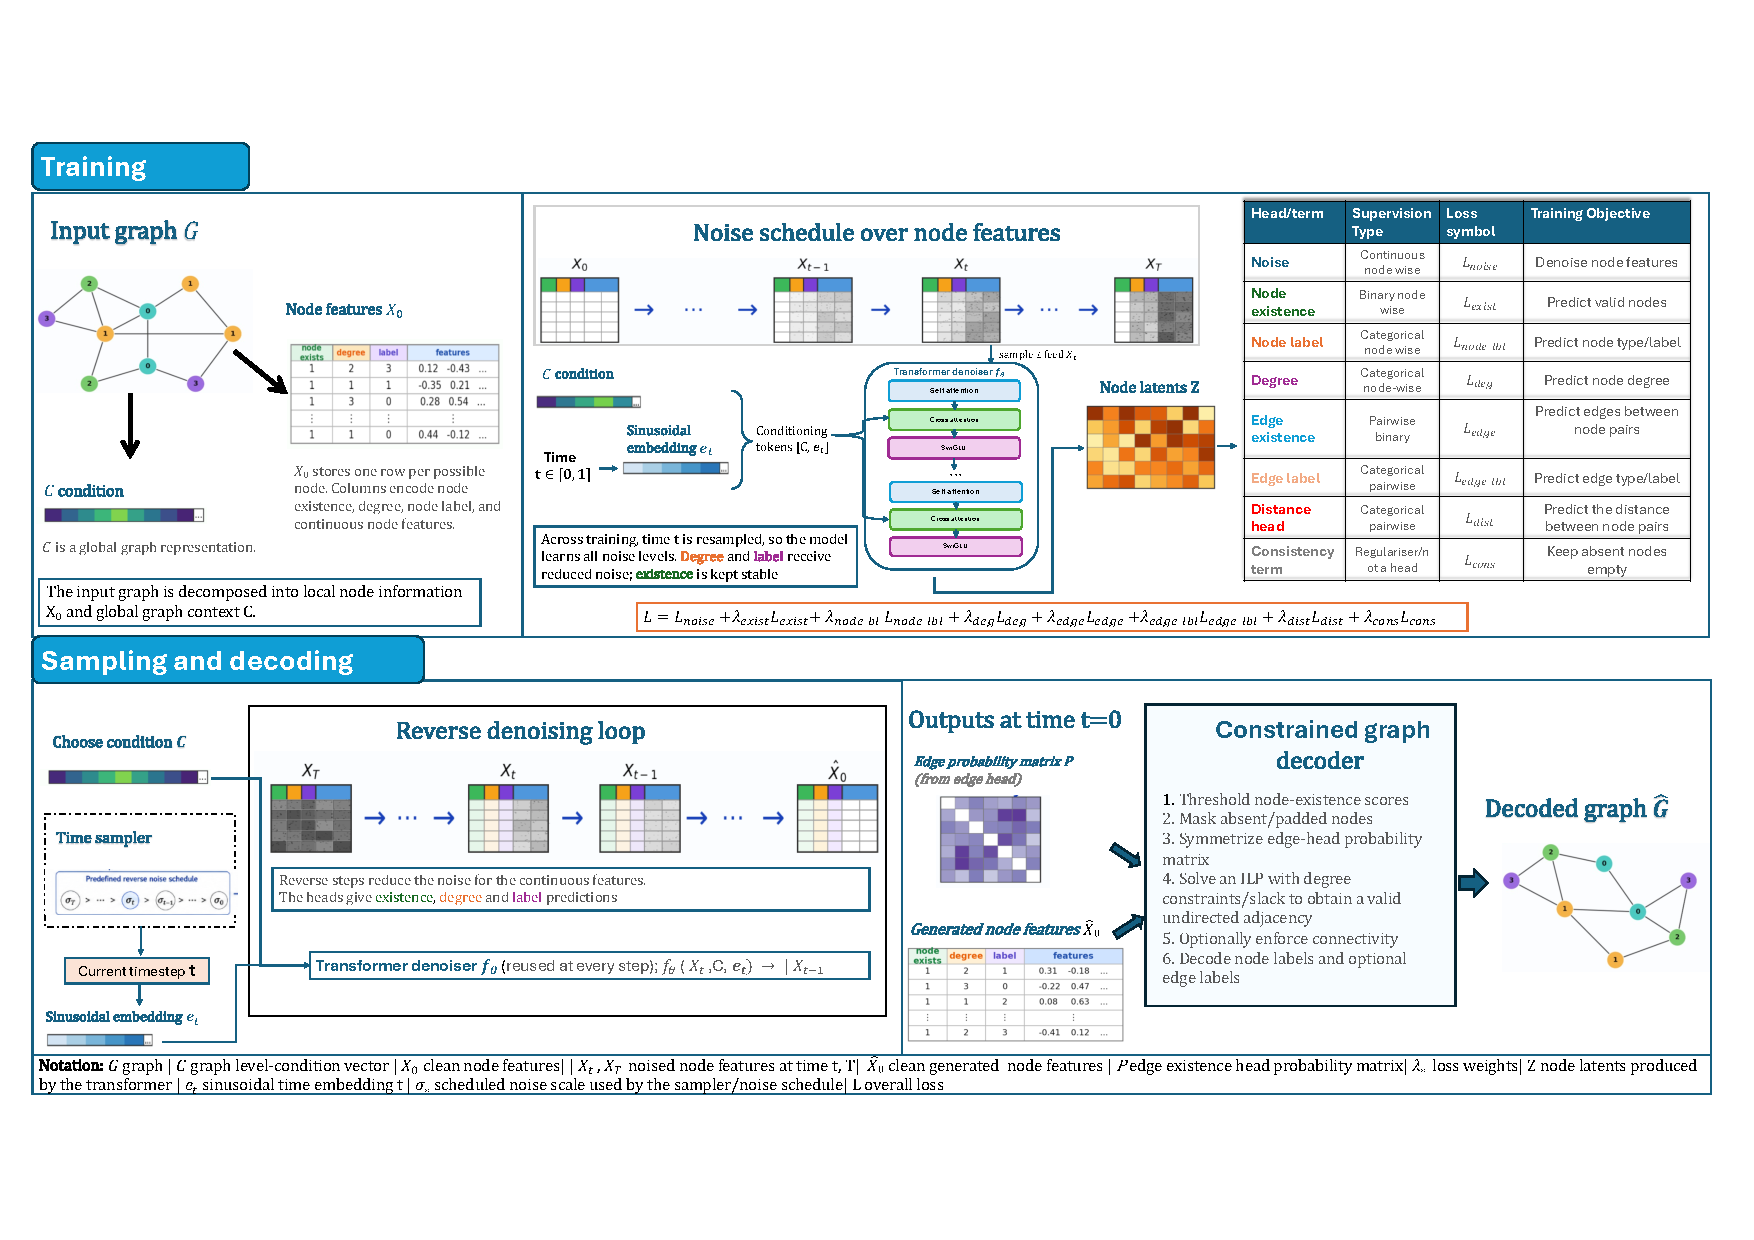
\includegraphics[
        width=1.35\textwidth,
        height=0.60\textheight,
        % keepaspectratio,
        trim=0cm 2cm 0cm 2cm, %left bottom right top
        clip
        clip,
        center=-3cm
    ]{images/diffusion/pipeine_generator.pdf}
    \caption{
    Overview of the proposed decompositional conditional denoising graph generator.
    The input graph is encoded into a node feature table $X_0$ and a graph-level condition
    vector $C$. During training, a time $t$ is sampled and noise is added to
    $X_0$ according to a column-wise schedule, producing $X_t$. The conditional
    transformer denoiser receives $X_t$, $C$, and the time embedding $e_t$, and
    produces node latents $Z$ used by node-wise and pairwise prediction heads.
    At sampling time, a reverse noise schedule is followed from $X_T$ to
    $\hat X_0$, reusing the same denoiser at each step. The generated node table
    and edge probability matrix are decoded into a valid graph by the constrained
    decoder.
    }
    \label{fig:generator:overview}
\end{figure}



\section{Encoding and Notation}
\label{sec:generator:notation}

Let \(G=(V,E)\) denote an input graph, where \(V\) is the set of nodes and
\(E\) is the set of edges. Each graph is represented by two encoders. A
graph-level vectorizer produces a conditioning vector

\[
C = \phi_G(G) \in \mathbb{R}^{d_C},
\]

where \(C\) is not the class target, but a continuous representation of the
whole graph. A node-level vectorizer produces a matrix

\[
X_0 \in \mathbb{R}^{N \times d_X},
\]

where \(N\) is the maximum number of node rows after padding and \(d_X\) is the
node-feature dimension. Each row corresponds to one possible node. In the
implementation, the first columns of each node row have special meanings:

\[
x_i = [m_i, d_i, \ell_i, r_i],
\]

where \(m_i \in \{0,1\}\) is the node-existence indicator, \(d_i\) is the node
degree, \(\ell_i\) is the node-label index, and \(r_i\) contains the remaining
continuous node features. Graphs with fewer than \(N\) nodes are padded with
rows whose existence indicator is zero.

The model can therefore handle variable-size graphs by learning which rows
represent real nodes. If fixed-size generation is desired, the training set can
instead be restricted to graphs with comparable node-count ranges.

Before training, node features and conditioning vectors are scaled. Continuous
tail features may optionally be reduced using PCA or truncated SVD, while the
existence, degree, and label columns are preserved explicitly.
Throughout the chapter, \(X_t\) denotes a noisy node table at time \(t\),
\(X_T\) denotes the high-noise endpoint, \(\hat X_0\) denotes the generated
clean node table, \(Z=Z^{(L)}\) denotes the final node latents, and
\(P=(p_{ij})\) denotes the edge-existence probability matrix. We write
\(\sigma_t=\sigma(t)\) for the scheduled noise scale and use
\(\lambda_{\ast}\) for loss weights.
\section{Forward Noising Process}
\label{sec:generator:forward}

At training time, a diffusion time value is sampled as

\[
t \sim \mathcal{U}(0,1).
\]

A time-dependent Gaussian perturbation is then applied to the clean node table:

\[
X_t = X_0 + S(t) \odot \epsilon,
\qquad
\epsilon \sim \mathcal{N}(0,I),
\]

where \(X_t\) is the noisy node table, \(S(t)\) is a feature-wise noise scale,
and \(\odot\) denotes element-wise multiplication. The scalar noise level is

\[
\sigma(t) = \sigma_{\min} + t(\sigma_{\max}-\sigma_{\min}).
\]

The degree and label columns receive reduced noise, controlled by
\texttt{noise\_degree\_factor} and \texttt{noise\_label\_factor}. This reflects
the fact that these columns represent discrete classes and are better handled
through classification heads than through continuous denoising.

\section{Conditional Transformer Denoiser}
\label{sec:generator:architecture}

The denoising network is a transformer model denoted by \(f_\theta\). It receives
the noisy node table \(X_t\), the graph-level condition \(C\), and the diffusion
time \(t\). The noisy node table is first normalized and projected into latent
tokens:

\[
H^{(0)} = W_X \mathrm{LN}(X_t) + b_X.
\]

The time value is converted into a sinusoidal embedding \(e_t\). The graph
condition \(C\) is projected into the same latent space. These two vectors form
memory tokens for cross-attention:

\[
M = [e_t, W_C C + b_C].
\]

Each transformer block applies self-attention across node tokens, cross-attention
to the memory tokens, and a feed-forward network with SwiGLU activation. After
\(L\) transformer layers, the final node latents are

\[
Z^{(L)} = f_\theta(X_t, C, t).
\]

Several prediction heads are attached to \(Z^{(L)}\). A continuous head predicts
the Gaussian noise \(\hat{\epsilon}\). Additional heads predict node existence,
degree classes, node-label classes, edge existence, edge labels, and hop-distance
classes when the corresponding supervision is available.

For edge prediction, the model uses a biaffine scorer. For node pair \((i,j)\),
with latent vectors \(z_i\) and \(z_j\), the edge logit is

\[
s_{ij} = z_i^\top U z_j + w^\top [z_i;z_j] + b.
\]

The edge probability is then

\[
p_{ij} = \sigma(s_{ij}).
\]

\section{Training Objective}
\label{sec:generator:training}

The model is trained with a weighted sum of reconstruction, classification, and
structural supervision losses. The continuous denoising loss is applied only to
real-valued feature columns and only to rows corresponding to existing nodes:

\[
\mathcal{L}_{\epsilon}
=
\frac{
\sum_{i} m_i
\left\|
M_{\mathrm{cont}} \odot
(\hat{\epsilon}_i - \epsilon_i)
\right\|_2^2
}{
\sum_i m_i + \delta
},
\]

where \(M_{\mathrm{cont}}\) masks out the existence, degree, and label columns,
and \(\delta\) is a small constant for numerical stability.

The existence loss is a binary cross-entropy loss:

\[
\mathcal{L}_{\mathrm{exist}}
=
\mathrm{BCEWithLogits}(\hat m_i, m_i).
\]

The degree and node-label losses are cross-entropy losses applied only to
existent nodes:

\[
\mathcal{L}_{\mathrm{deg}}
=
\mathrm{CE}(\hat d_i, d_i),
\qquad
\mathcal{L}_{\mathrm{lbl}}
=
\mathrm{CE}(\hat \ell_i, \ell_i).
\]

When edge supervision is enabled, the edge-existence loss is

\[
\mathcal{L}_{\mathrm{edge}}
=
\mathrm{BCEWithLogits}(s_{ij}, a_{ij}),
\]

where \(a_{ij}\) is the ground-truth edge indicator. If edge labels are available,
an additional edge-label cross-entropy loss may be used. The distance head, when
enabled, predicts hop-distance classes such as one-hop, two-hop, three-hop, and
four-or-more hops:

\[
\mathcal{L}_{\mathrm{dist}}
=
\mathrm{CE}(\hat h_{ij}, h_{ij}).
\]

A consistency loss penalizes nonzero continuous features on absent rows. Let

\[
\hat X_0 = X_t - S(t)\odot \hat\epsilon
\]

be the denoised estimate of the clean node table. The consistency term is

\[
\mathcal{L}_{\mathrm{cons}}
=
\sum_i (1-m_i)
\left\|
M_{\mathrm{cont}} \odot \hat x_i
\right\|_2^2.
\]

The total objective is

\[
\mathcal{L}
=
\lambda_{\epsilon}\mathcal{L}_{\epsilon}
+
\lambda_{\mathrm{exist}}\mathcal{L}_{\mathrm{exist}}
+
\lambda_{\mathrm{deg}}\mathcal{L}_{\mathrm{deg}}
+
\lambda_{\mathrm{lbl}}\mathcal{L}_{\mathrm{lbl}}
+
\lambda_{\mathrm{edge}}\mathcal{L}_{\mathrm{edge}}
+
\lambda_{\mathrm{dist}}\mathcal{L}_{\mathrm{dist}}
+
\lambda_{\mathrm{cons}}\mathcal{L}_{\mathrm{cons}}.
\]

In implementation, the existence, degree, label, and distance losses are weighted
by the diffusion noise level using

\[
w(t) = \frac{1}{\sigma(t)^2 + 10^{-4}},
\]

so that predictions at lower noise levels receive stronger supervision.

\section{Sampling Procedure}
\label{sec:generator:sampling}

At generation time, the model receives a conditioning vector \(C\). This vector
may be sampled from the empirical training-conditioning pool, obtained by
encoding an input graph, or produced by interpolation between conditioning
vectors.

Sampling begins from Gaussian noise:

\[
X_T \sim \mathcal{N}(0,I).
\]

The model then follows a decreasing sequence of noise levels
\(\sigma_T > \cdots > \sigma_0\). In the implementation, this sequence is based
on the Karras noise schedule \citep{karras2022elucidating}. At each step, the
model predicts the noise and performs a Heun-style predictor-corrector update.

\begin{algorithm}[H]
\caption{Conditional denoising graph generation}
\label{alg:generator:sampling}
\begin{algorithmic}[1]
\Require conditioning vector \(C\), number of steps \(T\)
\State Sample \(X_T \sim \mathcal{N}(0,I)\)
\State Construct decreasing noise levels \(\sigma_T,\ldots,\sigma_0\)
\For{\(k = T,\ldots,1\)}
    \State Convert \(\sigma_k\) to normalized time \(t_k\)
    \State Predict noise \(\hat\epsilon_k = f_\theta(X_k,C,t_k)\)
    \State Mask out existence, degree, and label columns from \(\hat\epsilon_k\)
    \State Euler prediction:
    \[
    X' = X_k - (\sigma_k-\sigma_{k-1})\hat\epsilon_k
    \]
    \State Predict corrected noise \(\hat\epsilon'\) at \(X'\)
    \State Heun correction:
    \[
    X_{k-1}
    =
    X_k
    -
    \frac{1}{2}(\sigma_k-\sigma_{k-1})
    (\hat\epsilon_k+\hat\epsilon')
    \]
\EndFor
\State Predict existence, degree, and label classes using the auxiliary heads
\State Inverse-transform the generated node table
\State Decode the node table into a graph
\end{algorithmic}
\end{algorithm}

The continuous denoising update is applied only to the continuous feature
columns. The existence, degree, and label columns are projected after sampling
using the trained auxiliary heads. Existence is obtained by thresholding the
existence probability, while degrees and labels are obtained by taking the
maximum-probability class. Degree predictions are also snapped to degree classes
observed among real training nodes.

\section{Graph Decoding and Constraint Handling}
\label{sec:generator:decoding}

The sampled node table is not yet a graph. It must be decoded into a valid
discrete structure. The decoder first determines which rows correspond to real
nodes using the existence indicator. Non-existent rows are removed.

For the remaining nodes, predicted degree classes are interpreted as target
degrees. Edge probabilities are obtained either from an external adjacency
classifier or, in the current implementation, from the generator's biaffine edge
head. The probability matrix is masked so that non-existent nodes cannot receive
edges, and it is symmetrized for undirected graph decoding.

The final adjacency matrix is obtained by solving a binary optimization problem.
Let \(a_{ij}\in\{0,1\}\) indicate whether an undirected edge is selected between
nodes \(i\) and \(j\). The decoder solves

\[
\max_{a}
\sum_{i<j} p_{ij}a_{ij}
-
\lambda_{\mathrm{slack}}
\sum_i (u_i+v_i),
\]

subject to degree constraints

\[
\sum_{j\neq i} a_{ij} + u_i - v_i = \hat d_i,
\]

where \(\hat d_i\) is the predicted target degree and \(u_i,v_i\) are slack
variables. When connectivity enforcement is enabled, additional flow constraints
are added so that the selected graph forms a connected component over the
existent nodes. The solver is warm-started using a maximum spanning tree over the
predicted edge probabilities.

After the adjacency matrix is decoded, node labels are recovered from the
generated label column or node-label head. Edge labels are decoded when an
edge-label head or edge-label classifier is available; otherwise, edges may be
returned without labels.

\section{Implementation Details}
\label{sec:generator:implementation}

The generator is implemented in PyTorch Lightning. The denoising backbone uses a
stack of cross-attention transformer layers. Each layer contains node-token
self-attention, cross-attention to condition and time tokens, and a SwiGLU
feed-forward network.

Training uses the Adam optimizer with a ReduceLROnPlateau learning-rate
scheduler. Early stopping and checkpointing are used when enabled. The training
data is split into training and validation subsets, and losses are logged for the
continuous denoising objective, existence prediction, degree prediction, label
prediction, edge supervision, and distance supervision.

The model supports optional dimensionality reduction of the continuous node
feature tail using PCA or truncated SVD. The first columns corresponding to
existence, degree, and label are kept explicitly because they are handled by
dedicated heads.

The decoder uses NetworkX for graph manipulation and PuLP with the CBC solver
for constrained adjacency optimization. This makes the final decoding step
explicit and interpretable: the neural model proposes node and edge quantities,
while the optimization layer enforces structural consistency.

\section{Discussion and Limitations}
\label{sec:generator:discussion}

The main advantage of the proposed generator is that it separates graph
generation into representation learning and constraint-aware decoding. The
denoising model learns a flexible conditional distribution over node tables,
while the decoder enforces important graph-level constraints such as node
existence, degree feasibility, symmetry, and optional connectivity.

However, the method also has limitations. First, decoding requires solving an
integer optimization problem, which can become expensive for large graphs.
Second, the model depends on the quality of the graph and node vectorizers; if
important structural information is not captured in these encodings, the
generator may not recover it. Third, because graphs are padded to a maximum
number of rows, generation quality may depend on the node-count range used during
training. For this reason, experiments should compare real and generated graphs
within comparable node-count ranges when the goal is to evaluate structural
fidelity.

Finally, although the model uses a diffusion-style denoising process, it differs
from graph diffusion models that directly diffuse adjacency matrices or discrete
edge types. The proposed approach is instead a decompositional conditional
denoising generator: it learns to generate node-level representations and then
uses a constraint-aware decoder to obtain valid graphs.
